The open, or once-through, fuel cycle is relatively simplistic and is in place
in most countries in the world currently utilizing nuclear power. In practice,
the primary fuel element used in this type of cycle is uranium; however, a
combination of thorium and uranium, or some other initial source of neutrons,
could be used in theory. The fuel cycle is considered open because fuel that is
used in a reactor is stored indefinitely once its reactivity has dropped below
useful levels due to the presence of neutron poisons, primarily in the form of
fission products.

Beginning the fuel cycle process, Uranium ore is initially extracted from the
ground using one of a variety of techniques including open pit mining,
underground mining, and \textit{in situ} leaching. The uranium ore is then
milled to form yellowcake, $\mathrm{U_3O_8}$. The tailings, or byproducts, of
this process are slightly radioactive and are therefore considered to be
low-level waste (LLW) by the Nuclear Regulatory Commission (NRC)
(see \citet{nrc_10_1985}).

Certain reactors are designed to use naturally enriched uranium. For these
reactors, yellowcake can be directly reduced with oxygen to form naturally
enrich $\mathrm{UO_2}$. For the majority of power reactors, however, the uranium
must be enriched with higher-than-normal levels of uranium-235. In order to do
so, yellowcake is sent to a conversion facility, which converts it from
$\mathrm{U_3O_8}$ to $\mathrm{UF_6}$. The uranium hexaflouride is then enriched
to the required level in an enrichment facility, of which three classes exist:
gaseous diffusion, the original enrichment technology; centrifugal diffusion,
the current enrichment technology; and Atomic Vapor Laser Isotope Separation
(AVLIS), a newer technology not currently in commercial production. The enriched
uranium hexaflouride is then sent to a fuel fabrication facility where it is
returned to yellowcake form before being reduced to uranium oxide, similarly to
the process for natural uranium fuel. The uranium oxide is then sintered into
pellets and loaded into fuel assemblies to be placed in a reactor. This process
in conjunction with uranium mining is termed the 'front end' of the nuclear fuel
cycle.

Making the open fuel cycle unique, once fuel has been processed in a reactor, it
is cooled off in pools for a number of years, and then stored in dry casks
before eventually being sent to a final repository. The physical location of the
fuel may vary during dry cask storage between the reactor site or some other
interim storage site.

Graphically, the open fuel cycle is shown in Figure \ref{fig:open-cycle}.

\begin{figure}[]
  \begin{center}
    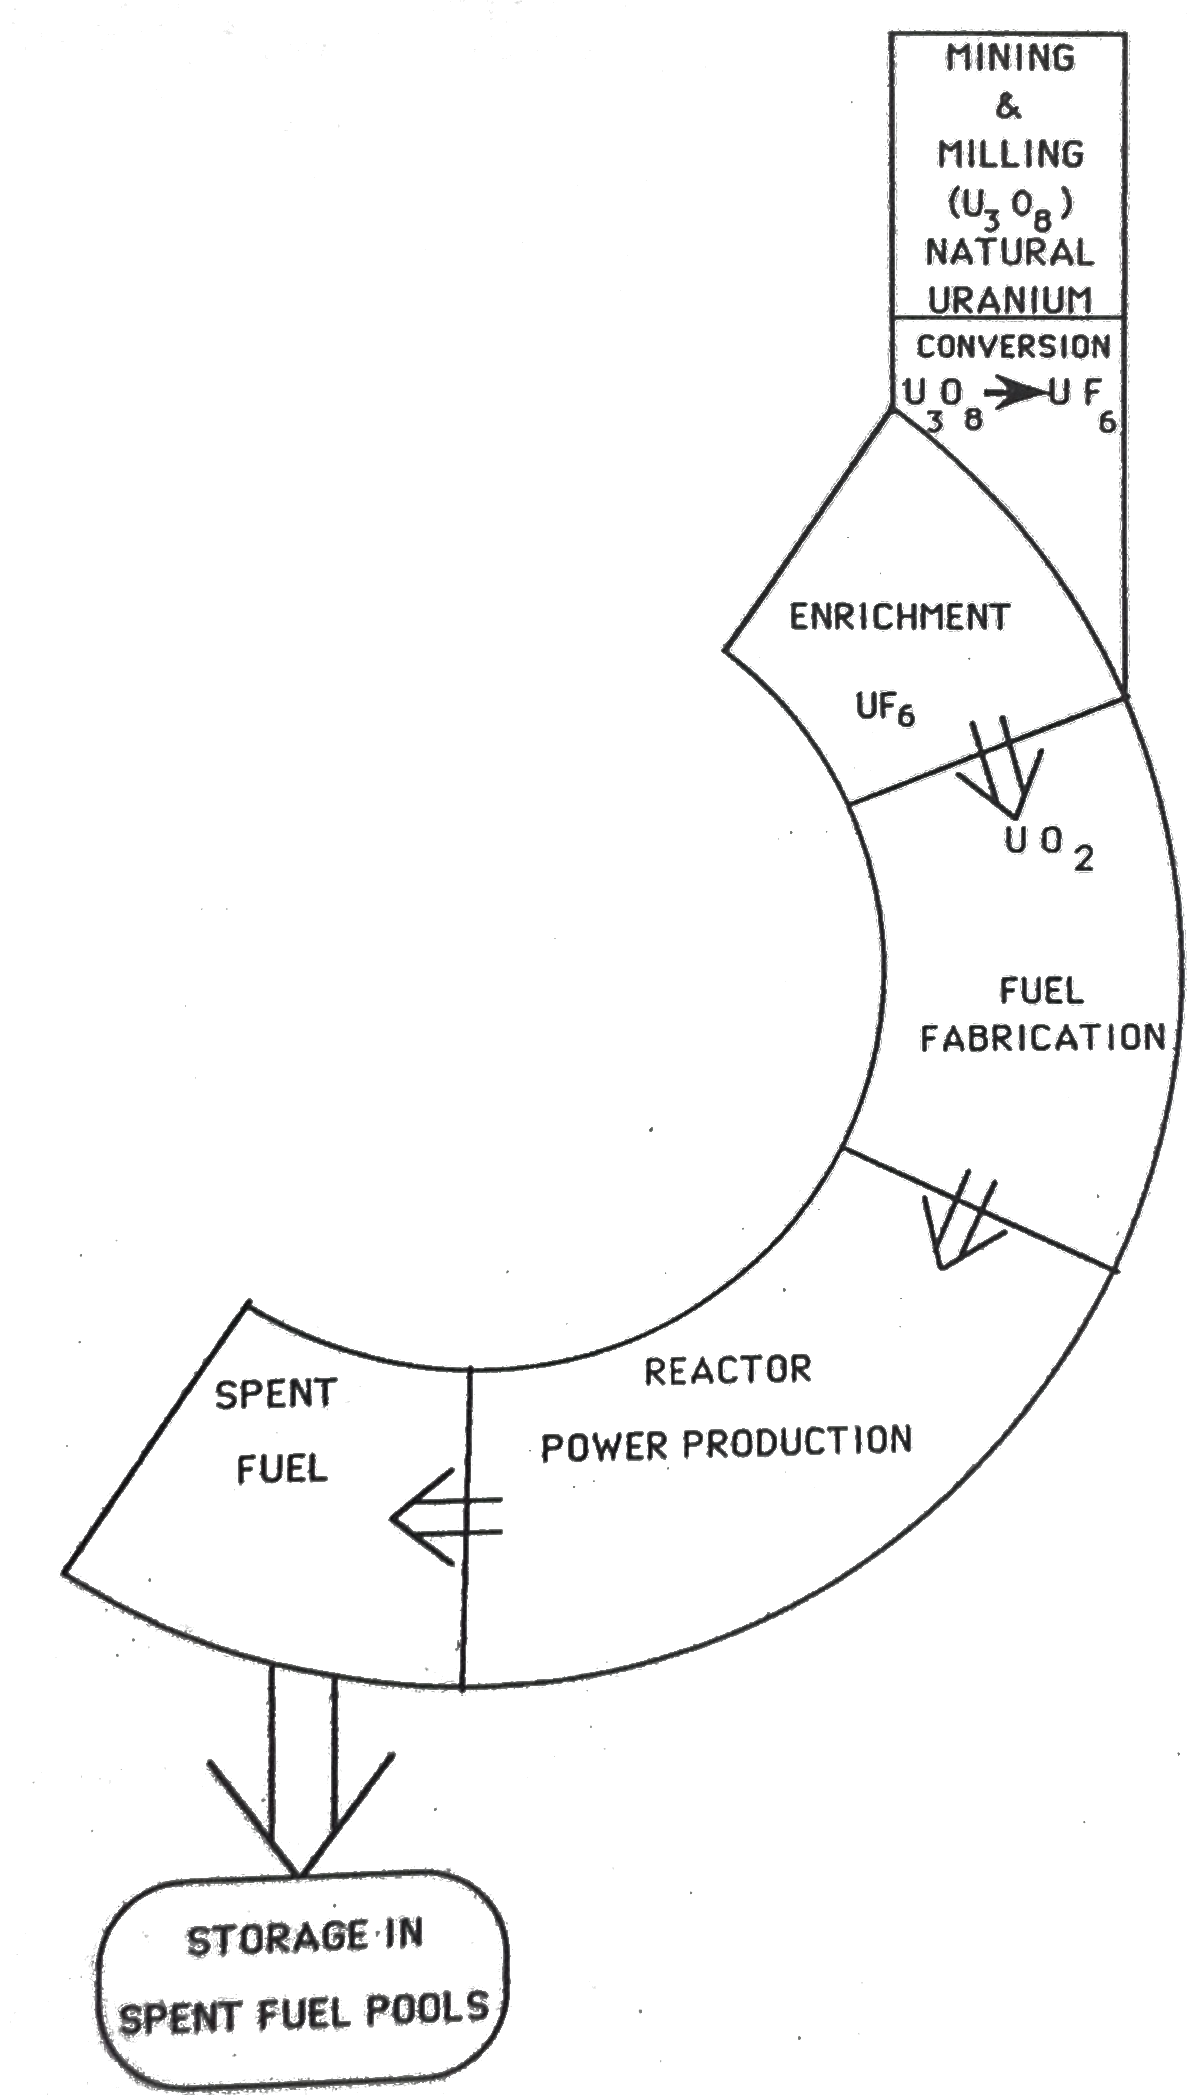
\includegraphics[width=4cm]{./chapters/intro/open_cycle.png}
  \caption{The once-through fuel cycle as shown in \cite{cochran1990nuclear}.}
  \label{fig:open-cycle}
  \end{center}
\end{figure}
